%!TEX root = thesis.tex
\chapter{Findings} % (fold)
\label{cha:findings}

% \crumbs
% {\textbf{Introduce chapter}}

While we have developed some idea of how software evolves, it is uncertain as to whether the same pressures apply to all aspects of a software system. In order to understand how the pressures of evolution relate to the vocabulary within source code, we set out to answer the following questions:

% \begin{itemize}
% 	% Growth-related questions
% 	\item What are the trends for growth in total size of the vocabulary across evolving software systems? Does this match findings for the growth of software systems as a whole?
% 	% Distribution-related questions
% 	\item What is the distribution of term usage frequency within vocabulary?
% 		\begin{itemize}
% 			\item Is there an observable similarity in the vocabulary distribution profiles between systems?
% 		\end{itemize}
% 	\item How does the distribution of term usage change throughout the evolution of a system?
% 		\begin{itemize}
% 			\item Are the most popular continually re-used?
% 			\item Are changes to the vocabulary stable or erratic?
% 		\end{itemize}
% 	\item Does the age of a term have an influence on the likelihood that it will be re-used?
% 	\item What do the most frequently used terms refer to? Are these terms related to the domain or architectural concepts (such as idioms and design patterns)?
% \end{itemize}

In this chapter, we address the above questions in order to gain a greater understanding of the nature of evolving source code vocabularies in open source software systems.

The rest of this chapter is organised as follows:

\crumbs{\textbf{Chapter structure}}

\section{Growth in Vocabulary} % (fold)
\label{sec:growth_in_vocabulary}

Lehman's laws argue that evolving software systems tend to exhibit sub-linear growth rate. This argument is based on the assumption that as software evolves its complexity increases but the overall effort towards development remains stable. Studies by Lehman \cite{Lehman97a} show that increases in complexity are caused both by the size of the system (volumetric complexity) as well as the internal complexity of some of the modules. The argument proposed by Lehman that the growth of evolving software systems is sub-linear has been supported by case studies observing system growth \cite{DAmbros07a, Gall97a, Lehman97a}. Despite this, studies of Open Source Software Systems have found evidence that linear and super-linear growth rates are also possible \cite{Godfrey01a,Israeli09a,Succi01a}.

What are the trends for growth in total size of the vocabulary across evolving software systems? Does this match growth exhibited by evolving software systems as a whole?

\subsection{Measuring Rate of Growth} % (fold)
\label{sub:measuring_growth_in_vocabulary}

To measure the amount of growth exhibited by a vocabulary we plot the total number of terms (i.e. vocabulary size) against the age of the systems (i.e. number of days since the initial version), for each version of the software system. We then fit a model of regression to the plotted values in order categorise the pattern of vocabulary growth as either a linear or quadratic (sub-linear or super-linear), depending on which is the most appropriate fit for the values.

For a comparison between the growth in vocabulary and system size (comprised of the sum of the number of bytes for each class within a version), we fit a model of regression to the values for system size to determine if there was a match between the two.

As the vocabulary and system size operate at differing scales, we plot the percentage of growth relative to the inital version of the system, allowing for a more apporiate comparison of the rates of growth. This approach to comparing growth follows that which was used in \cite{Paulson04a}.

\crumbs{\textbf{Mix-in}}

To determine the growth rate of vocabulary, we categorised the rate of growth according to the most appropriate regression model that fit the vocabulary size across versions. These possible growth rates, along with their associated implications are highlighted in Table~\ref{tab:vocab_growth_rate_implications}. A \emph{Sub-Linear} growth rate indicates that the vocabulary is unable to sustain growth, possibly due to an inability of developers to manage the linguistic overhead that is associated with introducing a large number of new terms, a characteristic expected of a system in which the core design undergoes refinement, but is conceptually stable. Meanwhile, a \emph{Super-Linear} growth rate would suggest that the system's architecture facilitates extension, possibly through the use of a plugin architecture, allowing new terms to be introduced without impacting the core design of system and introducing complexity.

% subsection measuring_growth_in_vocabulary (end)

\subsection{Observations of Growth} % (fold)
\label{sub:observations_of_growth}

\subsubsection{Patterns of Growth} % (fold)
\label{ssub:patterns_of_growth}

The vocabulary used within source code is fundamental to developers in facilitating program comprehension. As software evolves, developers must introduce new terms related to the concepts supporting continualy functional growth. However, the impact of evolution on the size of the vocabulary and whether it faces the same pressures as an evolving software system as a whole is not yet known.

In this study, we investigated the growth rate of the vocabulary in order to ascertain if the sub-linear growth rate expectation extends to vocabulary.

\begin{table*}[t]
\centering
\begin{tabular}{|p{.23\textwidth}|p{.72\textwidth}|}
\hline
{\bf Growth Rate} & {\bf Implications}\\
\hline
\hline
Sub-Linear
&
Developers are unable to increase the number of terms, due to the associated complexity that comes through introduction of concepts. This type of growth is expected in systems that do not easily allow extension, and are instead based around a core design that undergoes maintenance and refinement. 
\\
\hline
Super-Linear
&
Developers are able to continually increase the rate of term addition while managing the associated linguistic overhead. This type of growth is expected in systems which facilitate extension of functionality without altering the systems' core design (e.g. plug-in architectures).
\\
\hline
Linear
&
Developers are able to maintain a consistent rate of introducing new terms.
\\
\hline
\end{tabular}
\vspace{0.2cm}
\caption{The possible growth rates that may be exhibited by a vocabulary as it evolves, and the implications that are associated with these growth types.}
\label{tab:vocab_growth_rate_implications}
\vspace{-0.2cm}
\end{table*}

\begin{figure}[t]
\centering
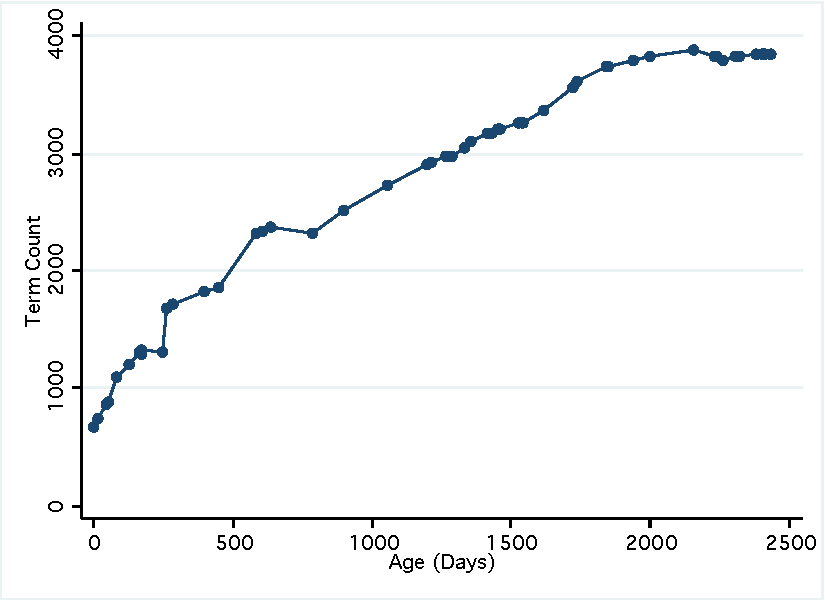
\includegraphics[width=\textwidth]{Figures/Vocab-AzureusGrowth.pdf}
\caption{The vocabulary size across the release history of Azureus, exhibiting sub-linear growth. There is a high growth rate in early versions, followed by a period of stable additions in subsequent versions. The latest releases show minimal vocabulary growth.}
\label{fig:vocab-growth-azureus}
\end{figure}

Of the 34 systems analysed, 28 (82\%) of the systems showed a sub-linear vocabulary growth rate, 3 (9\%) were linear and 3 (9\%) were super-linear. Despite the fact that the sub-linear growth rate is not universal, it was clearly the predominant and most likely growth rate amongst the systems we analysed. A common sub-linear growth pattern is highlighted in Figure~\ref{fig:vocab-growth-azureus}, which shows the vocabulary growth for Azureus. In the early versions of Azureus (ages 0--600), the vocabulary increases at a high rate to support fundamental concepts within the system. However, as it continues to evolve (ages 800--1700), the growth of the vocabulary slows as less terms are being added between releases. The latest releases (ages 1800--2500) show that significant growth in the size of vocabulary is no longer occurring. This result is most common amongst the systems analysed and favours the extension of Lehman's law relating to increasing complexity to an evolving vocabulary.

Although the growth rate of the vocabulary provides us with some insight into how it grows,
we refined our investigation by combining the this information with the overall system size growth. That is, we wanted to find out if vocabulary growth matches the overall size growth rate of the software system.

\begin{table*}[t]
\centering
\begin{tabular}{|p{.19\textwidth}|p{.19\textwidth}|p{.04\textwidth}|p{.48\textwidth}|}
\hline
{\bf Vocabulary} & {\bf System Size} & {\bf \#} & {\bf Implication} \\
\hline
\hline
Sub-Linear
&
Sub-Linear
&
19
&
Both system size and vocabulary size are being impacted by increasing complexity.
\\
\hline
Sub-Linear
&
Linear
&
8
&
Vocabulary is not being extended to support further functional growth.
\\
\hline
Sub-Linear
&
Super-Linear
&
1
&
Vocabulary is sufficient in representing concepts related to the increasing rate of functional growth.
\\
\hline
Linear
&
Linear
&
1
&
System size and vocabulary have not yet been impacted by complexity.
\\
\hline
Linear
&
Super-Linear
&
2
&
System is being extended without requiring a matching rate of growth in vocabulary.
\\
\hline
Super-Linear
&
Super-Linear
&
3
&
Both vocabulary and system size are being extended to support functional growth (likely via a plug-in architecture).
\\
\hline
\end{tabular}
\vspace{0.2cm}
\caption{Number of systems demonstrating particular combinations of vocabulary and system size growth rates, along with the implication for systems possessing these combinations.}
\label{tab:growth_rate_results}
\vspace{-0.2cm}
\end{table*}

\subsubsection{Vocabulary vs. System Size} % (fold)
\label{ssub:vocabulary_vs_system_size}

Plotting the system size (measured in the number of bytes that make up the version) and determine the most appropriate fit revealed a strong similarity in the growth of system size and vocabulary, as highlighted in Table~\ref{tab:growth_rate_results}. Overall, 23 (68\%) of the systems were found to have a rate of growth of vocabulary that matched that of the system size. Of the systems that were found to have matching growth rates, there was a noticeable similarity between the system size and vocabulary in terms of how both are impacted across versions. This similarity is illustrated in Figure~\ref{fig:comparative_growth_pmd}, which shows the vocabulary and system size growth rates for PMD.

Our findings that there is often a match in growth trends for the vocabulary and system size indicates that the absolute size growth exhibited by a system is a somewhat reliable predictor of the kind of growth that can be expected of the vocabulary.

Despite the similarities that are present, growth in system size does not serve as a direct indicator of how the vocabulary will go. While it is apparent that the two follow roughly similar patterns, there appears to be some variation from version to version.

\begin{figure}[t]
\centering
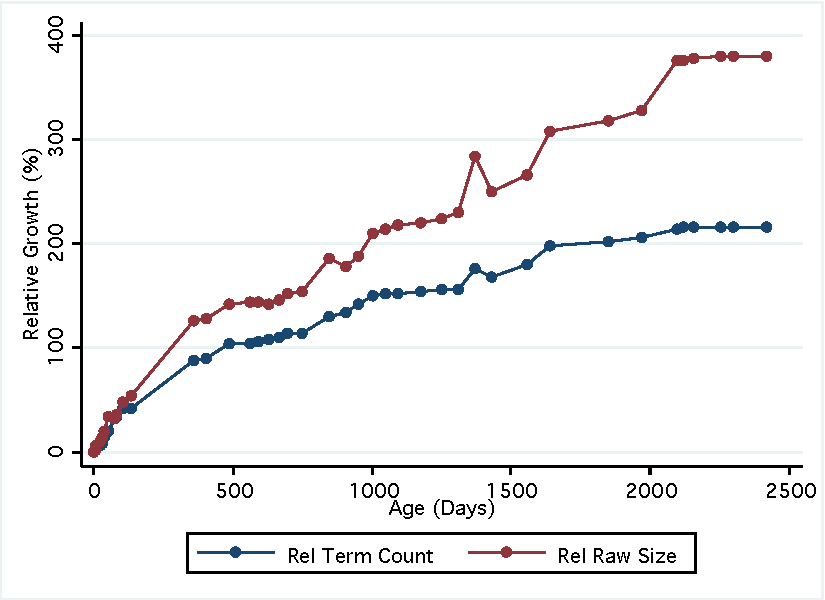
\includegraphics[width=\textwidth]{Figures/Vocab-PMDComparativeGrowth.pdf}
\caption{Relative growth for vocabulary and raw size for PMD. Although the raw size is increasing at a greater rate than the vocabulary, there is a clear similarity in the patterns of growth exhibited.}
\label{fig:comparative_growth_pmd}
\end{figure}

Software system vocabularies appear to, in general, be reaching a level of maturity at a particular stage of their evolution, as shown by the results showing predominately sub-linear growth. This suggests, that the further growth of the software is being supported by core concepts that are already present within the vocabulary. However, in cases in which the vocabulary was showing growth that was not sub-linear, this was matched by a similar growth rate for system size. The implication of this is that new terms are being added to the vocabulary in order to support functional growth that is evident from the increase in system size.

Predictably, based on what we know of how software systems evolve, the growth of vocabulary is far more substantial in earlier versions of software. This suggests that vocabulary as a whole is still in its infancy at this time, requiring expansion as time goes on in order to represent concepts within the system. As the software evolves, it appears as though vocabulary contains sufficient terminology for the developers to express themselves within the code and instead favour re-use of existing terms. The re-use of terms is discussed further in Sections~\ref{sec:changes_in_distribution} and ~\ref{sec:the_role_of_age_in_term_re_use}.

% subsubsection vocabulary_vs_system_size (end)

\section{Distribution of Vocabulary} % (fold)
\label{sec:distribution_of_vocabulary}

\subsection{Measuring Distribution of Vocabulary} % (fold)
\label{sub:measuring_distribution_of_vocabulary}

To measure how vocabulary is distributed throughout the system we plotted the frequency distributions for the number of times a term occurs within the source code.

Using this, we observed the similarity between the between the distribution profiles across all of the systems to determine if there was a pattern as to how vocabulary was distributed within source code.

% subsection measuring_distribution_of_vocabulary (end)

\subsection{Distribution Profiles} % (fold)
\label{sub:distribution_profiles}

What is the distribution of term usage frequency within vocabulary? Is there an observable similarity in the vocabulary distribution profiles between systems?

Studies of software systems involving the analysis of software metrics have shown that software is not normally distributed, but rather, exhibits a highly skewed distribution. Observing this trend of skewed software metrics, \textbf{Vasa} found that developers tend to prefer to deal with a small number of complex abstractions within software systems, rather than distributing this complexity throughout the system.

In this study, we investigated the how term usage within source code is distributed, to determine whether there is a tendency for developers to use a subset of the vocabulary with greater frequency than the rest of the vocabulary.

Plotting the frequency in which terms were used, we observed that a small number of terms had a far greater frequency of usage than the rest of the vocabulary. Applying the pareto principle, we set a threshold frequency value of 100 as the maximum frequency value to plot, whic accounted for approximately 95\% of the terms within the vocabulary. This allowed for greater readability of the charts of term frequency distribution.

The results showed that each of the systems analysed exhibited a remarkably similar distribution. The tendency was towards the usage of a substantial proportion of terms less than 5 times throughout the source code, as highlighted in Figure~\ref{fig:vocab-freq-dist-groovy}, which shows the term frequency distribution for Groovy. In contrast to this, a small set of terms are used with much greater frequency than the remainder of the vocabulary. A comparison of the distribution profiles between 4 of the systems analysed is shown in Figure~\ref{fig:vocab-freq-dist-comparison}.

Although a thorough analysis was not conducted, a comparison between the term frequency distribution for vocabulary and that of a natural-language document, revealed a similarly inequal distribution of terms. Figure~\ref{fig:vocab-freqdist-gadfly} shows the term frequency distribution for \emph{The Gadfly}, a novel by Ethel Lilian Voynich, which was published in 1897. While \emph{The Gadfly} exhibited a slightly more skewed distribution in favour of using terms with less frequency, it's distribution profile was almost identical to that which was found in the systems we analysed.

These findings indicate that developers tend to use a lot of terms within the vocabulary sparingly, while a small number of terms are constantly re-used. We suggest that the large proportion of terms that are used sparingly are applied in a supplementary context and are generally of low importance in comprehension of the system. Meanwhile, the most frequently used terms are concepts that are core to the system in question and hold significant semantic value. The types of terms used most frequently is discussed further in Section~\ref{sec:mining_the_domain_model}.

\begin{figure}[t]
\centering
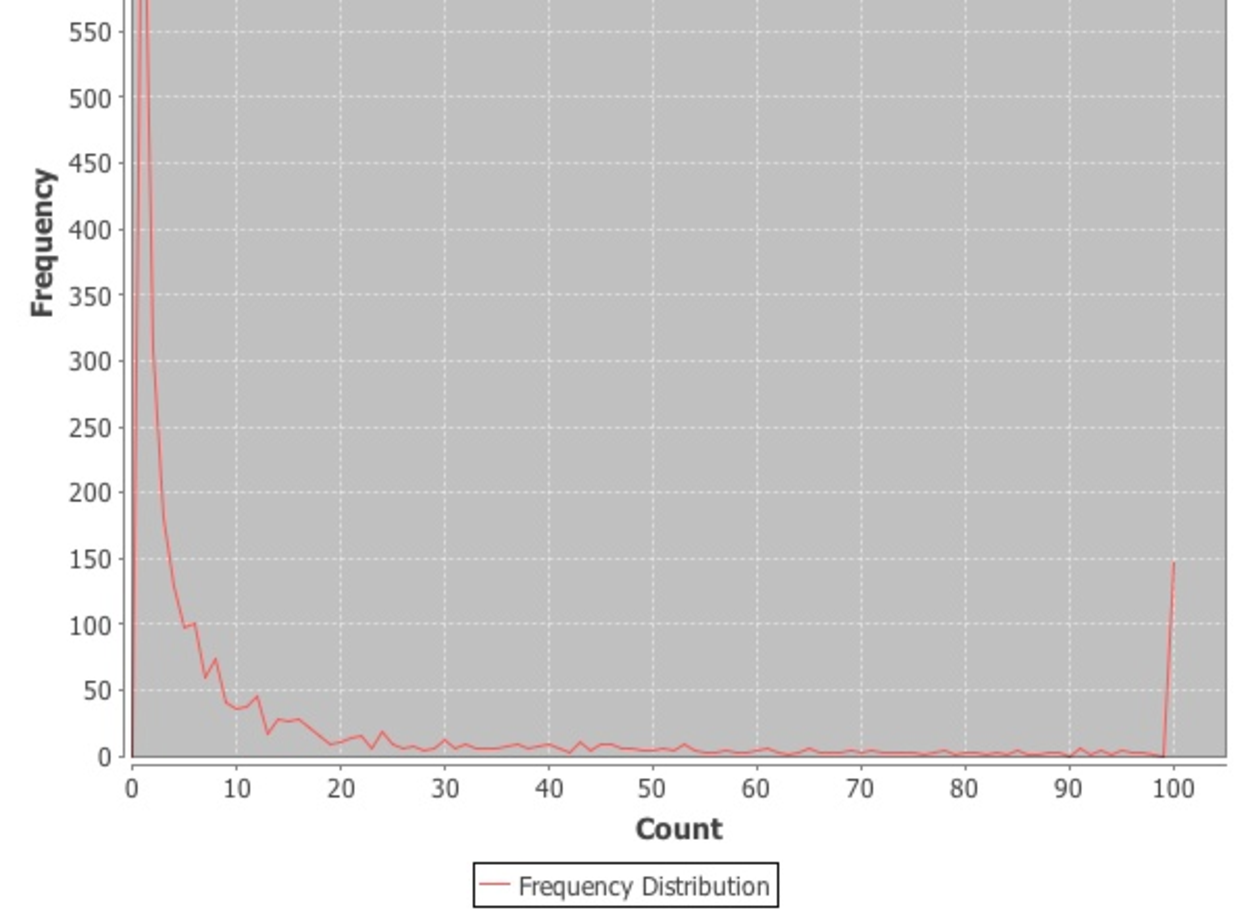
\includegraphics[width=\textwidth]{Figures/Vocab-GroovyFreqDist.pdf}
\caption{Term frequency distribution for Groovy, demonstrating a high skew towards using terms only a small number of times.}
\label{fig:vocab-freq-dist-groovy}
\end{figure}

\begin{figure}[t]
\centering
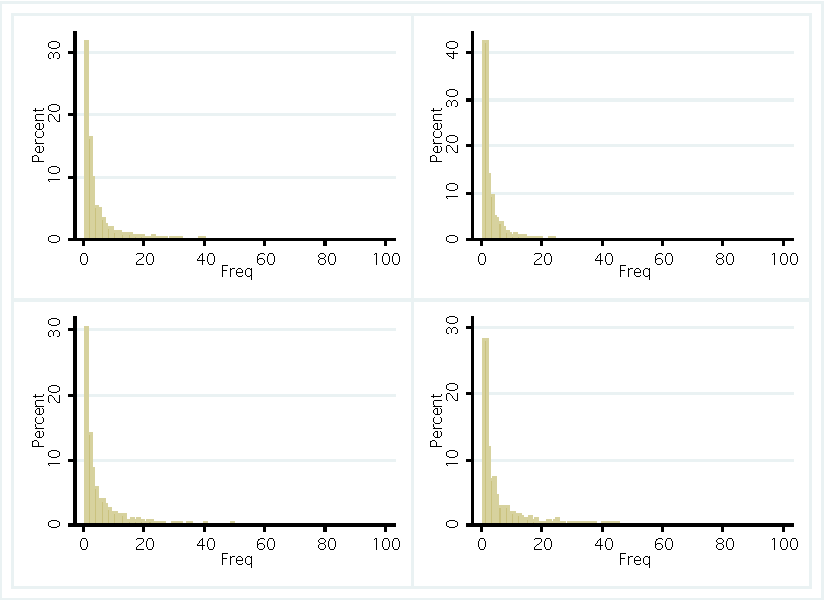
\includegraphics[width=\textwidth]{Figures/Vocab-FrequencyDistComparison.pdf}
\caption{Term frequency distributions for Groovy, PMD, JabRef and Spring. Each of the distribution profiles show an obvious tendency towards the usage of a substantial number of the terms less than 5 times.}
\label{fig:vocab-freq-dist-comparison}
\end{figure}

% subsection distribution_profiles (end)

% section distribution_of_vocabulary (end)

\section{Changes in Distribution} % (fold)
\label{sec:changes_in_distribution}

\subsection{Detecting Changes in Distribution} % (fold)
\label{sub:detecting_changes_in_distribution}

To determine whether developers favour the re-use of terms that are already popularly used, we examined how the usage frequency changes between subsequent releases of a software system.

A measure that has been used effectively in summarising abnormally distributed data is the Gini Coefficient, a value between 0 and 1 which describes the inequality of the distribution of wealth within a given population. A value of 0 is indicative of an equal distribution of wealth within a population (i.e. each member of the population has the same wealth), while in contrast, a value of 1 demonstrates perfect inequality (i.e. one individual accounts for all wealth).

Previous studies of software evolution have applied this measure in highlighting the abnormal distribution of software metrics and how this changes over time \cite{Vasa09a}. These studies found that a change in the value of the Gini of $\pm$0.04 indicates a significant shift in the distribution of wealth, providing a trigger for further investigation. 

To examine the distribution of wealth within vocabulary, we calculated the Gini Coefficient using the number of times a given term is used as an indicator of wealth.

% subsection detecting_changes_in_distribution (end)

\subsection{Vocabulary Distribution Changes} % (fold)
\label{ssub:vocabulary_distribution_changes}

Is the usage frequency for vocabulary consistent throughout the evolution of a system or do some terms attain greater popularity than others? Are the changes in frequency stable or erratic?

Lehman's law of continuing change argues that a software system must undergo regular adaption else become progressively less satisfactory. Studies investigating the change in software systems have shown support for continuing change in software, however the changes that occur typically are incremental and big changes are uncommon, indicating that software systems are stable as a whole.

Vocabulary is a crucial component in problem comprehension and the development of mental models. Although mental models are capable of adapting to change, a large magnitude of change can be highly disruptive and adaptation is more effective when change is brought about gradually.

In this study, we investigate the nature and magnitude of change in source vocabularies to determine if vocabulary follows the same pattern of stability as that of the software system as a whole.

\subsubsection{The Rich Get Richer} % (fold)
\label{sub:the_rich_get_richer}

Our results showed there is a high inequality in the distribution of wealth within source code vocabulary, with the Gini Coefficient values falling within a range of 0.57 and 0.86 for any version in any of the systems analysed. Figure~\ref{fig:vocab-gini-azureus} shows the Gini Coefficient values for the term distribution within the vocabulary of Azureus throughout its evolution. As shown, Azureus starts with a value of 0.67, indicating that there is at that point already a highly skewed distribution in the vocabulary. As of the latest version, the Gini has reached a value of 0.84, an overall increase of 0.17.

\begin{figure}[t]
\centering
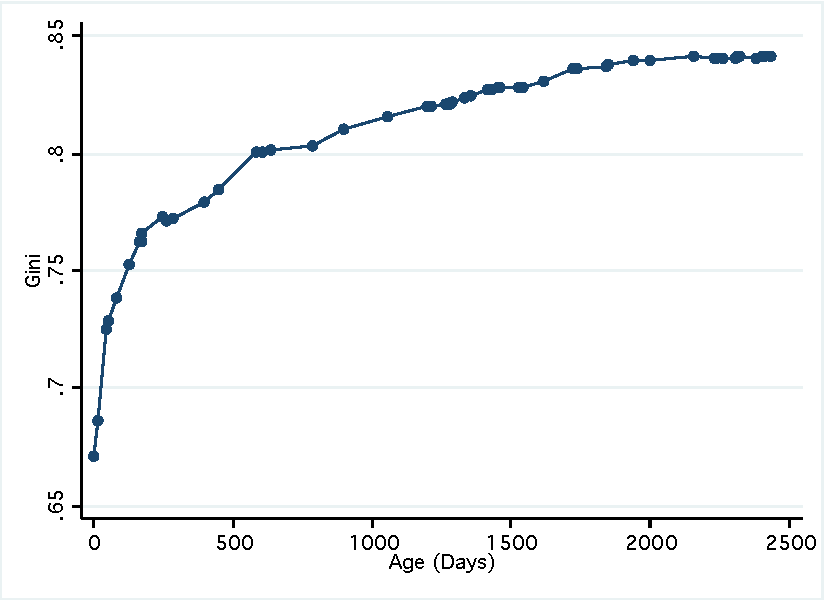
\includegraphics[width=\textwidth]{Figures/Vocab-AzureusGini.pdf}
\caption{Evolution of the Gini Coefficient of term usage for Azureus. The evolution shows most change occurs in early versions and stability is brought about over time.}
\label{fig:vocab-gini-azureus}
\end{figure}

Observing the evolution of the Gini Coefficient across all of the systems we analysed a similar trend emerges. Figure~\ref{fig:vocab-gini-rsn20-box} shows the box plots for the Gini for each of the systems we analysed through 20 versions of evolution. The plots show that the Gini continues to increase throughout evolution, a trend which continues even in the later versions of the systems.

\begin{figure}[t]
\centering
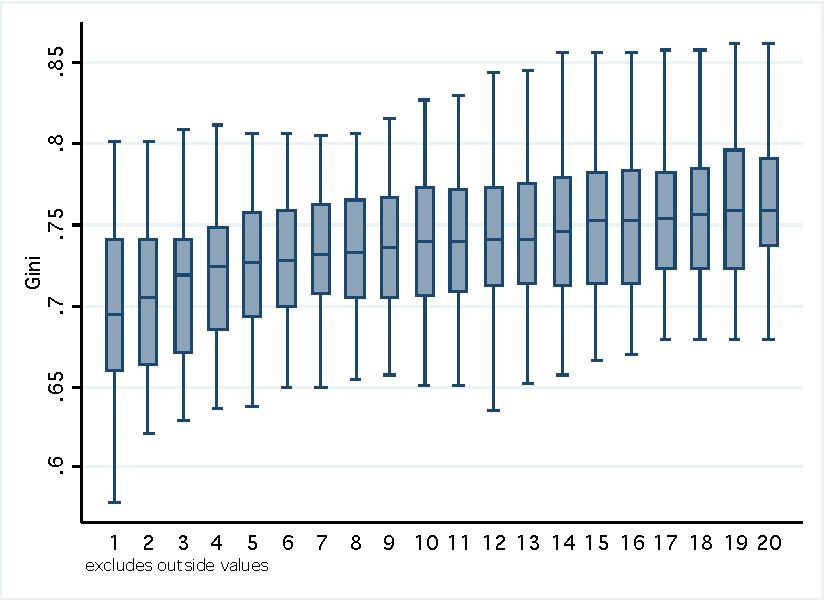
\includegraphics[width=\textwidth]{Figures/Vocab-RSN20GiniBox.pdf}
\caption{Box plots of the Gini Coefficient across 20 releases of the software systems. The plots show there is a continuing increase in Gini across releases, indicate the rich are getting richer.}
\label{fig:vocab-gini-rsn20-box}
\end{figure}

Comparing the Gini Coefficient values for initial and latest versions of the systems there is a noticeable shift in the range within which the Gini falls. This is illustrated in Figure~\ref{fig:vocab-firstlastgini-dist} shows the frequency distribution for the Gini Coefficient values for the first and last versions for each of the systems analysed. Looking at this plot, we can see there is a shift in the range of Gini values from 0.58--0.8 to 0.7--0.86.

\begin{figure}[t]
\centering
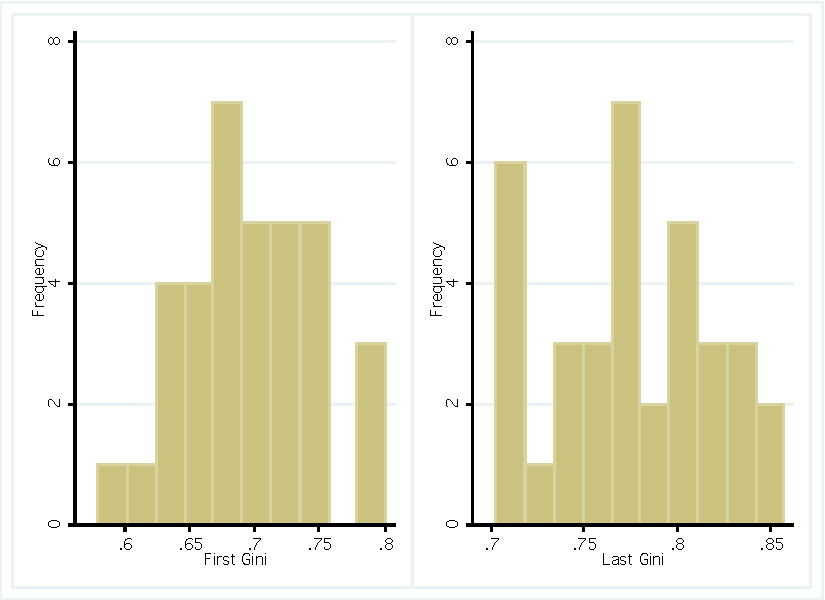
\includegraphics[width=\textwidth]{Figures/Vocab-FirstLastGini.pdf}
\caption{Distribution of the Gini Coefficient values for the first and last versions of each of the systems analysed. The distributions show an increase in the range within which Gini values fall within.}
\label{fig:vocab-firstlastgini-dist}
\end{figure}

When we calculate Spearman's Correlation Coefficient for each of the systems between the Gini  Coefficient and age of each version in the system, the results show there is a strong correlation between the two, as illustrated in Figure~\ref{fig:vocab-gini-spearman}. 25 (73\%) of the systems have a Spearman value greater than 0.9, which matches the overall trend highlighted in Figure~\ref{fig:vocab-gini-rsn20-box}.

While the results were highly skewed in favour of strong postive correlations, there was a couple of noticeable exceptions. Flow4J exhibited a relatively weak correlation of 0.236, resultant of inconsistent increases and decreases in the distribution of wealth as measured by the Gini. A relatively large decrease (0.015) in the Gini between versions 0.8.0 and 0.9.0 resulted in a wealth distribution similar to that of initial versions of the system.

KoLmafia was another system that laid outside of the majority, with a correlation of 0.6. Looking at the changes in Gini over time, there is an alternating trend in which a number of versions exhibit an increasing Gini, followed by a number of versions in which it decreases. A possible cause for this could be the continued introduction of new terms to the vocabulary that have substantial wealth, indicating that the vocabulary is adapting to significant changes over multiple versions.

Quartz was the only system to exhibit a negative correlation, yielding a value of -0.341. This was caused by a steady decrease from the initial Gini value for the first few versions of Quartz, followed by alternating increases and decreases in the Gini for later versions.

The exact cause of the relatively weak and negative correlations could not be determined. Given that the trend is overwhelmingly towards an increasing Gini, there are obviously underlying drivers at play that precipitate this different behaviour. What these drivers are and whether there are any implications for the lack of a strong correlation is an open topic for further study.

\begin{figure}[t]
\centering
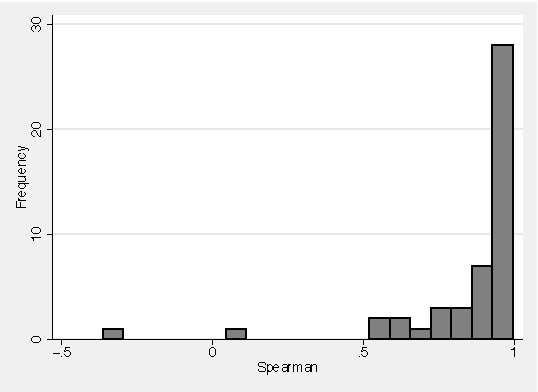
\includegraphics[width=\textwidth]{Figures/Vocab-GiniSpearmanFreqDist.pdf}
\caption{Gini Coefficient Spearman Correlation frequency distribution. Most systems show a strong correlation, though there are some exceptions.}
\label{fig:vocab-gini-spearman}
\end{figure}

Our findings indicate that the rich do get richer as a software system evolves. The high Gini values shown in more recent versions indicate that there are a small set of terms that are fundamental to the vocabulary present within the source code, and will inevitably be re-used. However, as these values seem to be bounded, we postulate that there are terms within the vocabulary that will see occasional heavy re-use, despite not being a core component of the vocabulary, which makes the richest terms relatively less wealthy.

% subsubsection the_rich_get_richer (end)

\subsubsection{Change is not Erratric} % (fold)
\label{ssub:change_is_not_erratric}

When we look at the amount of change that occurs in the Gini value between individual releases, we see that the overall the vocabulary is consistently stable between any two adjacent releases. This stability can be observed in Figure~\ref{fig:vocab-gini-delta-cumul}, which shows the cumulative distribution for Gini delta between two versions for all of the releases for each system we analysed. Approximately 90\% of the changes in Gini between two versions were less than 0.01 and 80\% less than 0.005, far less than 0.04 which was the value used to indicate that a significant change had occurred.

There were, however, some notable exceptions to the otherwise low Gini delta values, summarised in Table~\ref{tab:outstanding_gini_deltas}. Of all of the systems analysed, Ant had the highest delta between any two versions with delta of 0.0509 from version 1.1.0 to 1.2.0. As 1.2.0 was only the second release (RSN 2) of Ant, the substantial change was most likely the result of the application of vocabulary being erratic during early releases. This was also the case for Checkstyle version 3.1.0, which had a delta of 0.0462. Only two systems, Webwork and XWork, contained versions later in their release history that brought about a significant Gini change. In the case of both of these systems, the releases were a beta release of an upcoming major release which introduced a lot of new functionality. The substantial shift in the Gini values was resultant of the introduction of new terms to support this functional growth that possessed a large amount of wealth.

\begin{figure}[t]
\centering
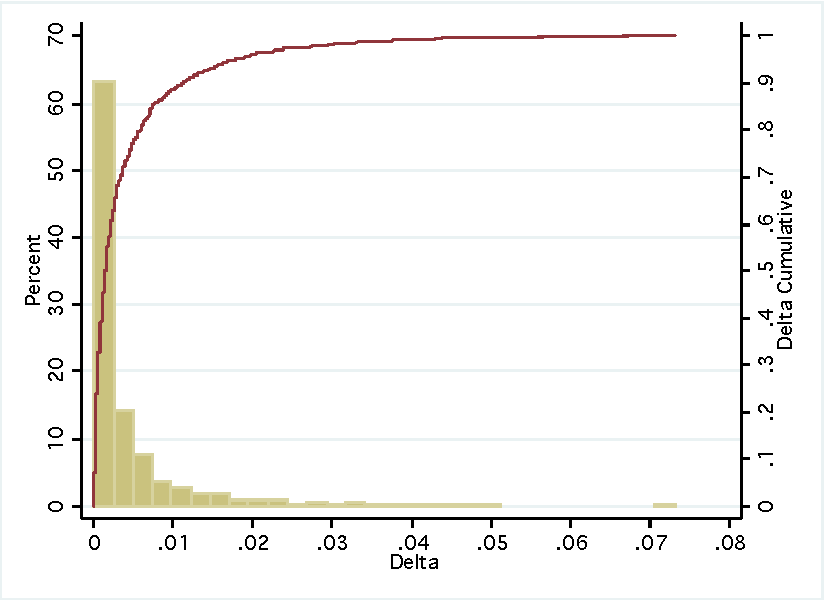
\includegraphics[width=\textwidth]{Figures/Vocab-GiniDeltaCumulFreq.pdf}
\caption{Cumulative distribution of Gini Coefficient deltas. The distribution reveals at 90\% of deltas are less than 0.01, implicating high stability.}
\label{fig:vocab-gini-delta-cumul}
\end{figure}

\begin{table*}[t]
\centering
\begin{tabular}{|p{.15\textwidth}|p{.09\textwidth}|p{.10\textwidth}|p{.50\textwidth}|}
\hline
{\bf System} & {\bf Ver.} & {\bf Delta} & {\bf Cause}\\
\hline
\hline
Ant
&
1.2.0
&
0.0509
&
Early release (RSN 2) of the software, usage of vocabulary is still erratic
\\
\hline
Checkstyle
&
3.1.0
&
0.0462
&
Early release (RSN 2) of the software, usage of vocabulary is still erratic
\\
% \hline
% Struts
% &
% 1.3.5
% &
% 0.0484
% &
% \textbf{Fill in}
% \\
% \hline
% Struts
% &
% 2.0.1
% &
% -0.0426
% &
% \textbf{Fill in}
% \\
\hline
Webwork
&
2.2b1
&
0.0465
&
Beta version of a major release introducing a lot of new functionality
\\
\hline
XWork
&
2.0b2
&
0.0444
&
Beta version of a major release introducing a lot of new functionality
\\
\hline
\end{tabular}
\vspace{0.2cm}
\caption{Significant changes in the Gini Coefficient between versions of the systems analysed and the causes for these big changes}
\label{tab:outstanding_gini_deltas}
\vspace{-0.2cm}
\end{table*}

Overall, our findings suggest that the distribution of vocabulary is very stable over time, with large changes occurring due to major versions which introduce terms that have a very high occurrence (this is not often). This suggests that while the software is evolving and being subjected to changes across releases, the stability of the vocabulary is generally well maintained and that the vocabulary is not being augmented to the point at which the mental model of developers is at threat to be seriously disrupted.

% subsubsection change_is_not_erratric (end)

% subsection vocabulary_distribution_changes (end)

% section changes_in_distribution (end)

\section{The Role of Age in Term Re-Use} % (fold)
\label{sec:the_role_of_age_in_term_re_use}

\subsection{Measuring the Influence of Age on Term Re-Use} % (fold)
\label{sub:measuring_the_influence_of_age_on_term_re_use}

To determine the influence that the age of a term had upon its likelihood of being re-used, we use the latest version of a system as the basis for its popularity, as this provided the most current view of the vocabulary. For each of the terms in the vocabulary, we calculate the age of any given term by determining the number of days since the version in which the term was first introduced. We take the age of a term and its popularity in the latest version and observe whether there is a monotonic relationship between the two. In the case where a monotonic relationship exists, this indicates that the age of a term is a direct indicator for it's likelihood for re-use. Where there is an inverse monotonic relationship, this tells us that new terms are much more likely to be re-used than older terms.

% subsection measuring_the_influence_of_age_on_term_re_use (end)

\subsection{The Likelihood of Term Re-Use} % (fold)
\label{sub:the_likelihood_of_term_re_use}

Does the age of a term have an influence on the likelihood it will be re-used? Do new features being introduced result in new supporting vocabulary that is used heavily or is there a tendency to re-use vocabulary that is already there?

Studies of software solution have shown that developers have a tendency to prefer to re-use existing abstractions within a software system, rather than create new ones. This is due to both the familiarity that developers have with these abstractions and the cognitive overhead associated with introducing complex new abstractions.

To determine whether familarity is preserved within vocabulary, we assessed the likelihood of a term being re-used based upon its age, to ascertain whether developers have a tendency to re-use terms that a introduced early in a systems lifetime or whether old terms are abandoned in favour of new terminology describing the functional evolution of the system.

Plotting the frequency with which terms are used against their age, a general trend emerges. The trend shows the terms within the vocabulary that have been present since the first version account for a large number of the most popular terms, while only a few terms that are introduced in later versions are used with high frequency. This trend is highlighted in Figure~\ref{fig:vocab-freqage-hibernate}, which shows the plot for Hibernate. Examining the terms that occur with high frequency that are introduced in later versions of the system, we notice that they relate to important concepts within Hibernate. In version 2.0.0, released 506 days after the initial version of Hibernate, the term \emph{criteria} is introduced, relating to a feature introduced allowing sophisticated queries of data from a database. Version 3.5.0 Beta 2 sees the introduction of the term \emph{audit}, relating to tracking the changes made to data within a database. Section~\ref{sec:mining_the_domain_model} further investigates the kind of terms that are used most frequently.

\begin{figure}[t]
\centering
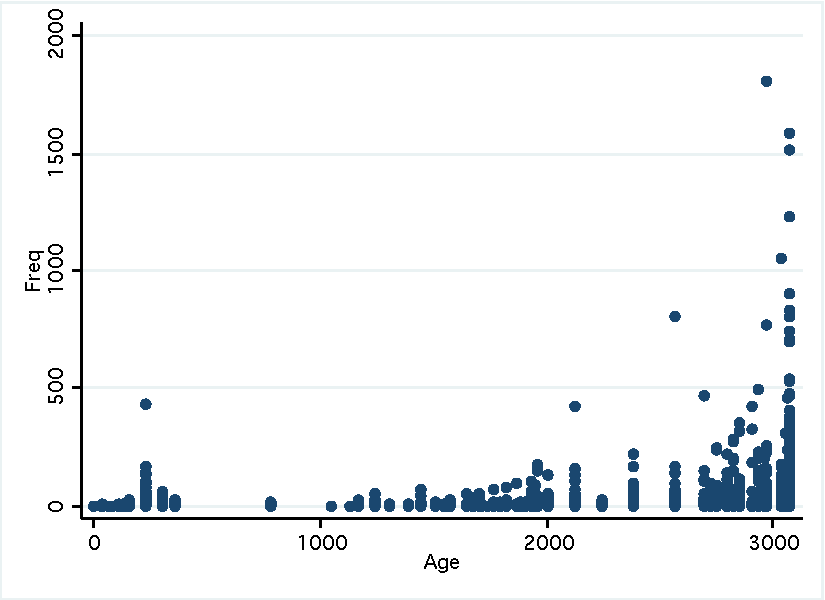
\includegraphics[width=\textwidth]{Figures/Vocab-HibernateFrequencyAge.pdf}
\caption{Plot of the term frequency vs. age based upon the popularity of terms in the latest version of Hibernate. The plot shows favour towards more frequent usage of older terms.}
\label{fig:vocab-freqage-hibernate}
\end{figure}

To get a more precise understanding of the relationship between term re-use and age, we calculated the Spearman's Correlation Coefficient of term frequency and age. Figure~\ref{fig:vocab-freqage-spearman-dist} shows the distribution of Spearman values across each of the systems. The results show that each of the systems analysed had a positive correlation, meaning that the age of a term has at least some influence on whether it will be re-used. The strength of the correlation, however, did vary across the systems, with a range of 0.13--0.61.

\begin{figure}[t]
\centering
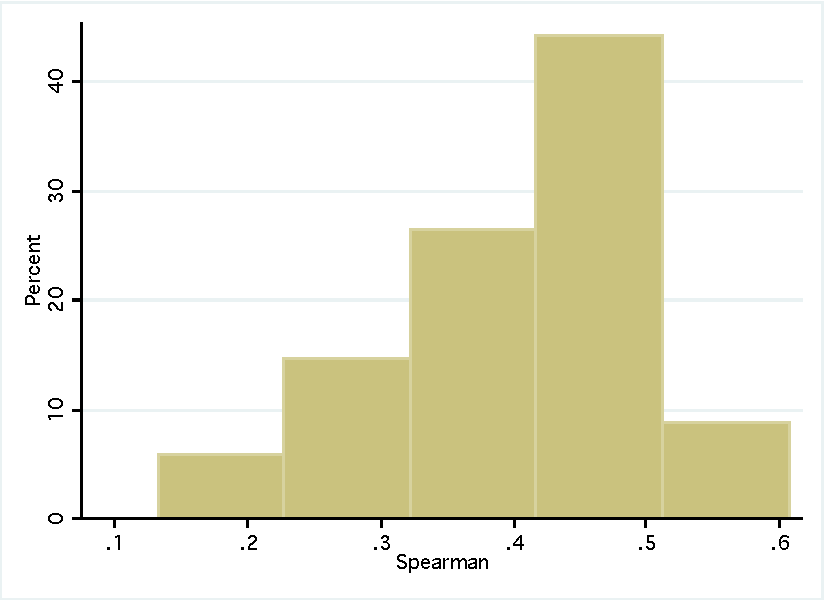
\includegraphics[width=\textwidth]{Figures/Vocab-FrequencyAgeSpearmanDist.pdf}
\caption{Distribution of the Spearman Correlation Coefficient values for frequency vs. age. The distribution shows there is a varied amount of corrletation between frequency and age across the systems.}
\label{fig:vocab-freqage-spearman-dist}
\end{figure}

These results indicate that most of the re-usable terms are established within early versions of system, forming the base of the vocabulary with which developers are able to communicate in their codebase. However, vocabularies do appear to be susceptible to the introduction of new terms throughout evolution that hold an importance in their own right, which is reflected by a high frequency of usage.

% subsection the_likelihood_of_term_re_use (end)

% section the_role_of_age_in_term_re_use (end)

\section{Mining the Domain Model} % (fold)
\label{sec:mining_the_domain_model}

What do the most frequently used terms within vocabularies refer to? Are they primarily pertaining to the software's domain, its design elements or something entirely different?

Best practices in software development suggest that programmers will write code that is communicative of the purpose and intention of the software system. When practising object-oriented programming, there are general guidelines that suggest how developers should reason about the design of their application, which allows them to build a solution around the problem they are trying to solve. These guidelines include the usage of a domain model, which captures the main entities within the problem space, as well as design patterns and idioms that represent re-usable concepts that can be applied to tailoring a system's architecture to suit the problem.

While these guidelines are in place to aid developers in the design and implementation of their applications, there is no governance with regard to how developers apply the vocabulary associated with them within their source code. While we can speculate that developers make use of domain related terms, it is uncertain as to whether developers actually utilise the vocabulary associated with these guidelines to good effect when writing code.

To determine whether developers effectively use domain-related terms within their source code's vocabulary, we extracted the 10 most popular terms from the latest version of each of the systems. In the following two sections, we investigate the terms most popularly used within Ant and Avasa.

\subsection{Case Studies} % (fold)
\label{sub:case_studies}

\subsubsection{Ant} % (fold)
\label{ssub:ant}

Looking at the top 10 most popularly used terms for Ant, we see that these terms are predominately related to the domain. We confirmed the meaning of each of these terms by observing the Ant user manual and other associated project documentation.

\crumbs
{
	\textbf{Put this in a table or something...}

	- project: Project definition
	
	- path: File system/URI paths
	
	- selector: Files can be selected based on criteria other than filename
	
	- zip: ZIP format, which Ant utilises a lot
	
	- filter: Apply filters to tasks
	
	- resource: External resource, such a file or URL, etc.
	
	- stream: I/O
	
	- task: Tasks within a build file
	
	- build: Manage building is what Ant does
	
	- execute: Used to perform tasks
}

Observing the usage patterns of these terms throughout Ant's evolution, presented in Figure~\ref{fig:vocab-popular-terms-ant}, we see that terms are typically re-used in bursts across a small number of versions, as opposed to a continual rate of re-use.

It is interesting to note that each of the 10 most popular terms have been present in the system since the initial version (1.1.0) and have consistently been amongst the most popularly used terms. This finding further supports the notion that developers conserve familiarity as presented in Sections~\ref{sub:the_rich_get_richer} and \ref{sec:the_role_of_age_in_term_re_use}, indicating that terms that hold a high level of semantic importance are not abandoned and replaced by new terminology.

\begin{figure}[t]
\centering
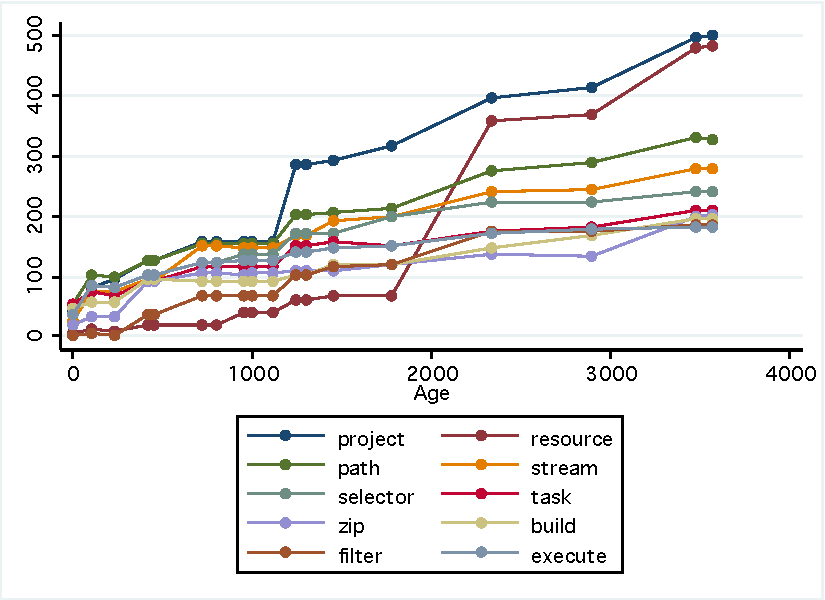
\includegraphics[width=\textwidth]{Figures/Vocab-AntPopular.pdf}
\caption{Evolution of the top 10 most popularly used terms in Ant}
\label{fig:vocab-popular-terms-ant}
\end{figure}

% subsubsection avasa (end)

\subsubsection{Avasa} % (fold)
\label{ssub:avasa}

Avasa is a simulation tool for air-traffic controllers which displays the flight routes for commercial aircraft. Taking the top 10 terms for Avasa, we can see that a number of these are clearly domain related.

\crumbs
{
\textbf{Put this in a table or something...}

- flight: Flight for an aircraft

- airport: Airport from which flights take off

- simulation: Concept of a simulation

- time: Simulation time

- waypoint: Geographical point that aircraft travel through

- date: Date

- filterable: Re-used concept relate to the able to filter 

- view: View (of MVC)

- model: Model (of MVC) (fields)

- mode: Indicator of state
}

Interestingly the usage patterns for the 10 most popular terms, shown in Figure~\ref{fig:vocab-popular-terms-avasa}, is similar to that which was observed for Ant in Section~\ref{ssub:ant}, in that the popular terms are re-used relatively heavily in a small number of versions and sparingly in others.

\begin{figure}[t]
\centering
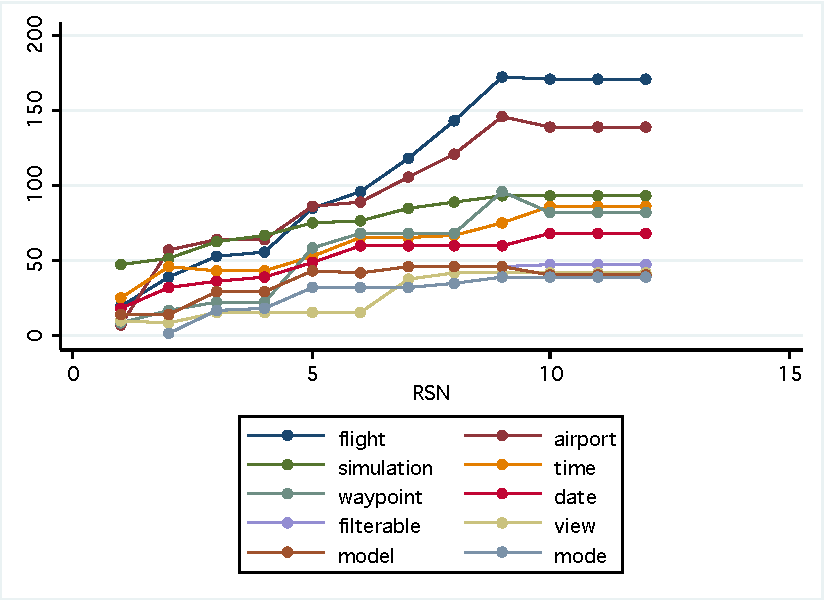
\includegraphics[width=\textwidth]{Figures/Vocab-AvasaPopular.pdf}
\caption{Evolution of the top 10 most popularly used terms in Avasa}
\label{fig:vocab-popular-terms-avasa}
\end{figure}

% subsubsection avasa (end)

% subsection case_studies (end)

% section mining_the_domain_model (end)

\section{General Discussion} % (fold)
\label{sec:general_discussion}

Overall, our findings show that vocabulary is highly concentrated within source code, a trend which is apparent even in early versions of the software. This tells us that developers place at least some guided thought into how they use vocabulary when the system is in early development. 

Once this vocabulary has been established early, the most popularly used terms typically increase in popularity incrementally over subsequent releases. This suggests that once the developers have formed a mental model of the system, it becomes increasingly unlikely that this will change as time goes on, as developers will try to conserve familiarity in the vocabulary by re-using the terms that have been present since the initial versions. The implication of this is that careful thought must be taken when establishing the vocabulary to ensure that it can adequately facilitate comprehension for the developers. If terminology is chosen hapharzardly, developers face the risk of being stuck with vocabulary that is inappropriate, which could lead to disrupted and/or inconsistent mental models held by developers working on the software.

While continued growth of the vocabulary throughout the evolution of a software system is evident, this growth typically follows the growth patterns of the software system as a whole, as is somewhat predictable. Although the amount of growth between versions can sometimes be quite large, the impact that this growth has upon the developers comphrension of the vocabulary is not necessarily proportional to the growth. In order to determine the effect of introducing new vocabulary, a sophisticated understanding of how new vocabulary is applied and how it relates to existing terminology is required in order to properly identify and communicate significant change.

Our investigations into the most popularly used terms revealed that developers make heavy use of domain-related and architectural concepts within the vocabulary. Although the popularity of a term seems to be indicative of its importance to the vocabulary and mental model of the developers, there may also be some terms that are less frequently used that are just as important. Interestingly, the trend appears to favour an increase in the use of these of terms across some, but not at all release. We suggest that major releases (i.e. those with the most functional growth) account for increases in these terms, as the terms are related to the concepts supporting the functionality that is being added or extended.

% section general_discussion (end)

% chapter findings (end)